\documentclass[a4paper,12pt]{article}
\usepackage[a4paper,top=1.3cm,bottom=2cm,left=1.5cm,right=1.5cm,marginparwidth=0.75cm]{geometry}
\usepackage{setspace}
\usepackage{cmap}		
\usepackage{amsmath,amsfonts,amssymb,amsthm,mathtools} 			
 				
\usepackage[T2A]{fontenc}			
\usepackage[utf8]{inputenc}			
\usepackage[english,russian]{babel}
\usepackage{multirow}
\usepackage{graphicx}
\usepackage{wrapfig}
\usepackage{subcaption}
\usepackage{tabularx}
\usepackage{float}
\usepackage{longtable}
\usepackage{hyperref}
\hypersetup{colorlinks=true,urlcolor=blue}
\usepackage[rgb]{xcolor}
\usepackage{icomma} 
\usepackage{euscript}


\DeclareMathOperator{\sgn}{\mathop{sgn}}
\newcommand*{\hm}[1]{#1\nobreak\discretionary{}
	{\hbox{$\mathsurround=0pt #1$}}{}}


\title{Калибровка RuO$_2$ термометра}
\author{Лавыгин Кирилл}
\date{\today}



\begin{document}

\maketitle

\begin{abstract}
В работе проведена калибровка термометра на основе RuO$_2$ резистора в диапазоне до 1.42 К. Для этого были использованы газовый термометр и термометр  на давлении насыщенных паров He$_4$. Для измерений использовался криостат откачки паров He$_4$.
\end{abstract}

\section{Оборудование}

В работе используются:
\begin{itemize}
    \item Криостат: азотный и гелиевый дьюары;
    \item Датчики «Baratron» для измерения давления газа в криостате и газовом термометре;
    \item Форвакуумный насос, гелиевый насос, сеть для сбора испаряемого гелия;
    \item Мультиметр «Keithley 2000»;
    \item Генератор «Juntek PSG9080».
\end{itemize}

\section{Подготовка к эксперименту}
Для автоматической записи экспериментальных данных в файл была создана программа в среде LabView.

Компьютер, на котором исполняется программа на LabView, принимает информацию от вольтметра, сигналы на который приходят от двух манометров «Baratron», образца RuO$_2$ и шунтирующего резистора. Номинал шунта был выбран сильно больше типичного сопротивления образца, чтобы ток через образец не сильно менялся при изменении сопротивления образца.

Также он задает напряжение на генераторе, которое определяет измерительный ток (генератор в данной работе использовался как генератор постоянного напряжения). Стоит заметить, что вольтметр, встроенный в генератор не используется для измерений, так как является неточным.
\begin{figure}[H]
    \centering
    \begin{subfigure}{0.48\textwidth}
        \centering
        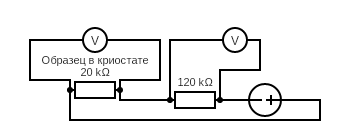
\includegraphics[width=\linewidth]{scheme.png}
        \caption{Схема измерительной цепи}
        \label{fig:sub1}
    \end{subfigure}
    \hfill
    \begin{subfigure}{0.48\textwidth}
        \centering
        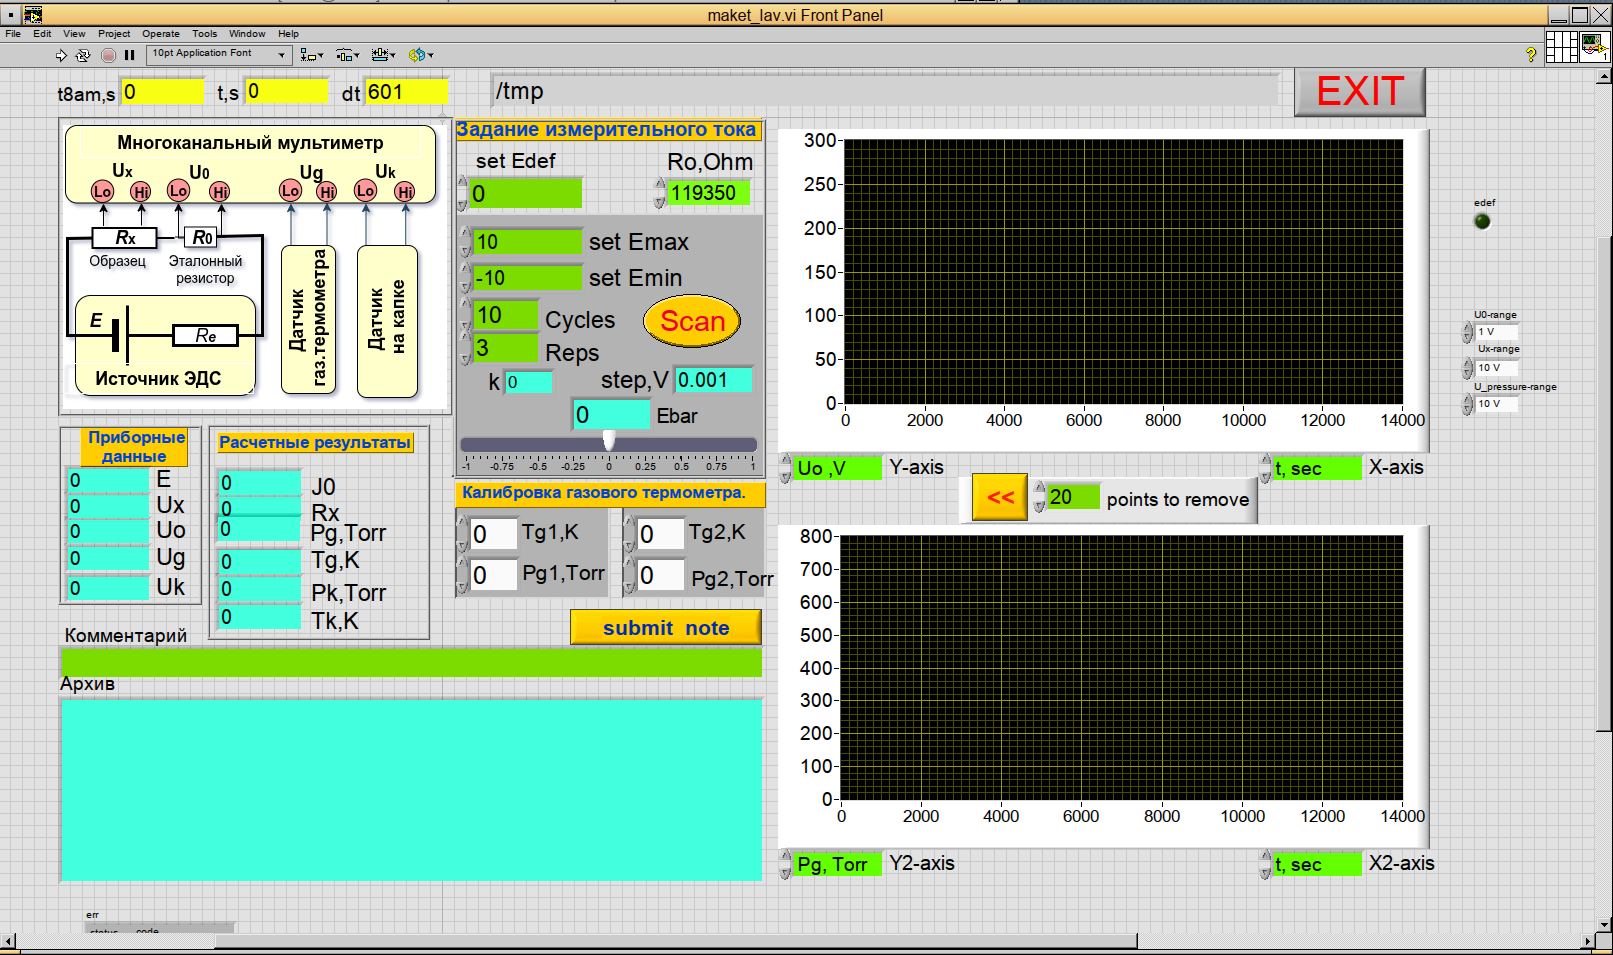
\includegraphics[width=\linewidth]{front_panel}
        \caption{Передняя панель программы LabView}
        \label{fig:sub2}
    \end{subfigure}
\end{figure}


\begin{figure}[H]
\centering
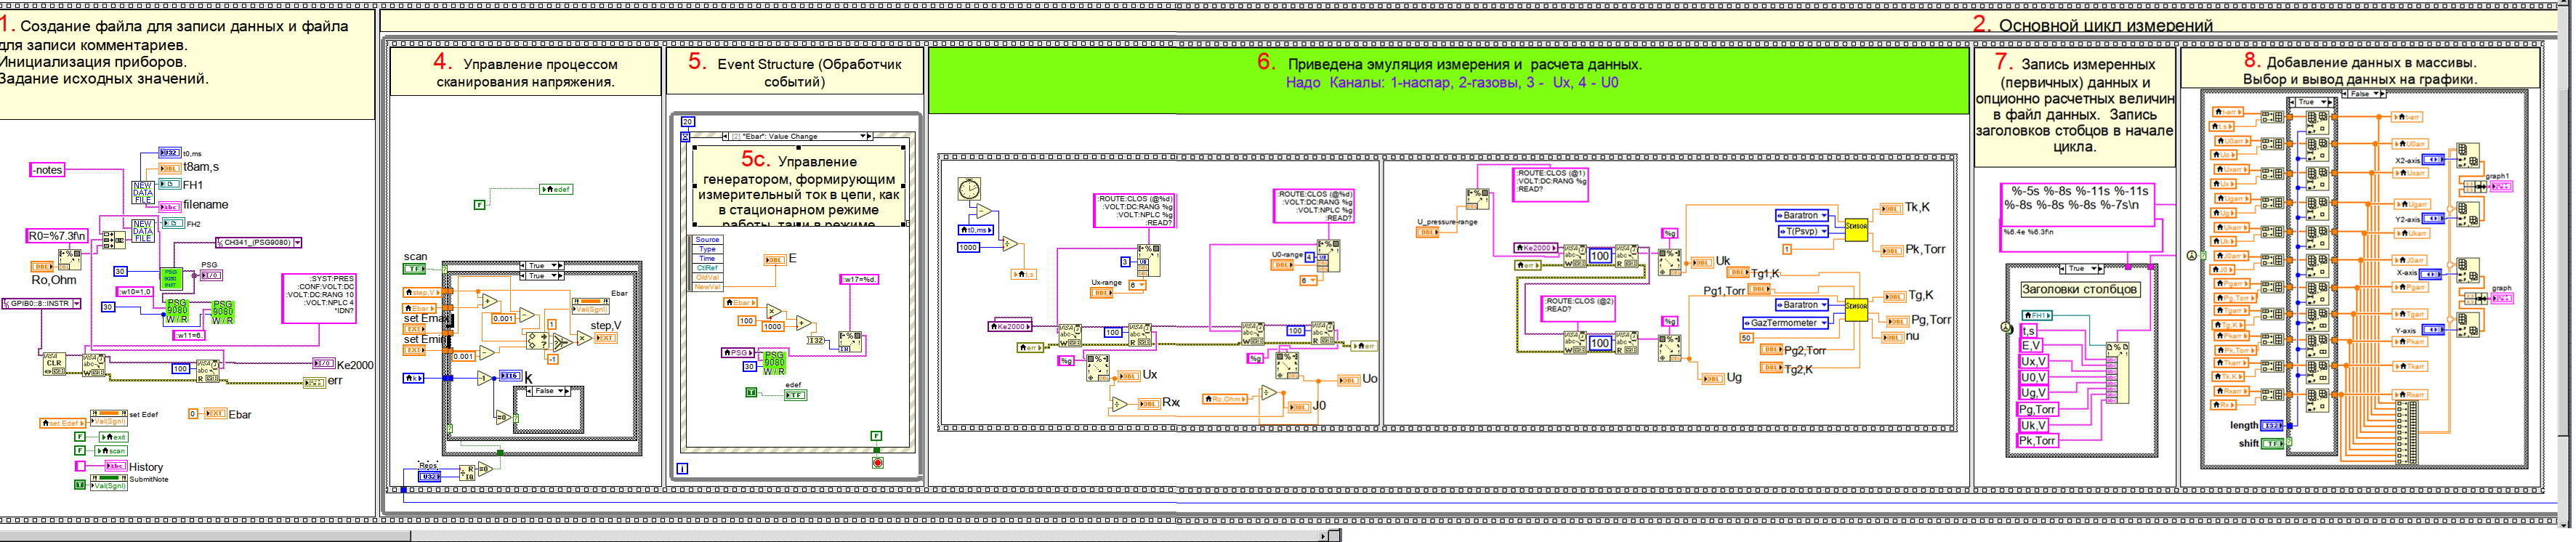
\includegraphics[width=\textwidth]{labview.png}
\caption{Программа в LabView}
\end{figure}

В качестве датчика мы будем калибровать SMD резистор номиналом 20КОм, изготовленный из RuO$_2$. Данные резистору имеют свойство сильно увеличивать свое сопротивление при низких температурах, так как серьезно падает возможность тунеллирования электронов между кристалликами внутри резистора. Мы размещаем резистор на вставке, используя клей БФ6, припаиваем контакты к выводам, которые ведут на 'голову вставки', помещаем вставку в герметичный гелиевый дьюар, а его в азотный.

\section{Эксперимент}

Сначала опишем производимый эксперимент. 
\subsection{Процесс эксперимента}
\begin{figure}[h]
    \centering
    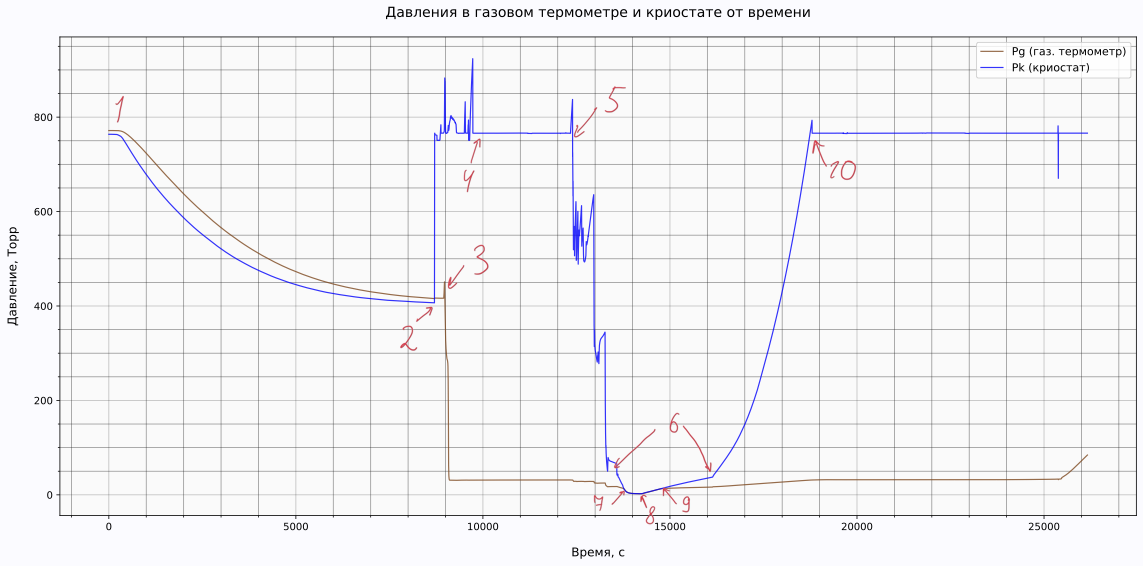
\includegraphics[width=\linewidth]{plot_pressures.png}
    \caption{Зависимость давлений в криостате и газовом термометре от времени на протяжении эксперимента}
\end{figure}
\begin{figure}[h]
    \centering
    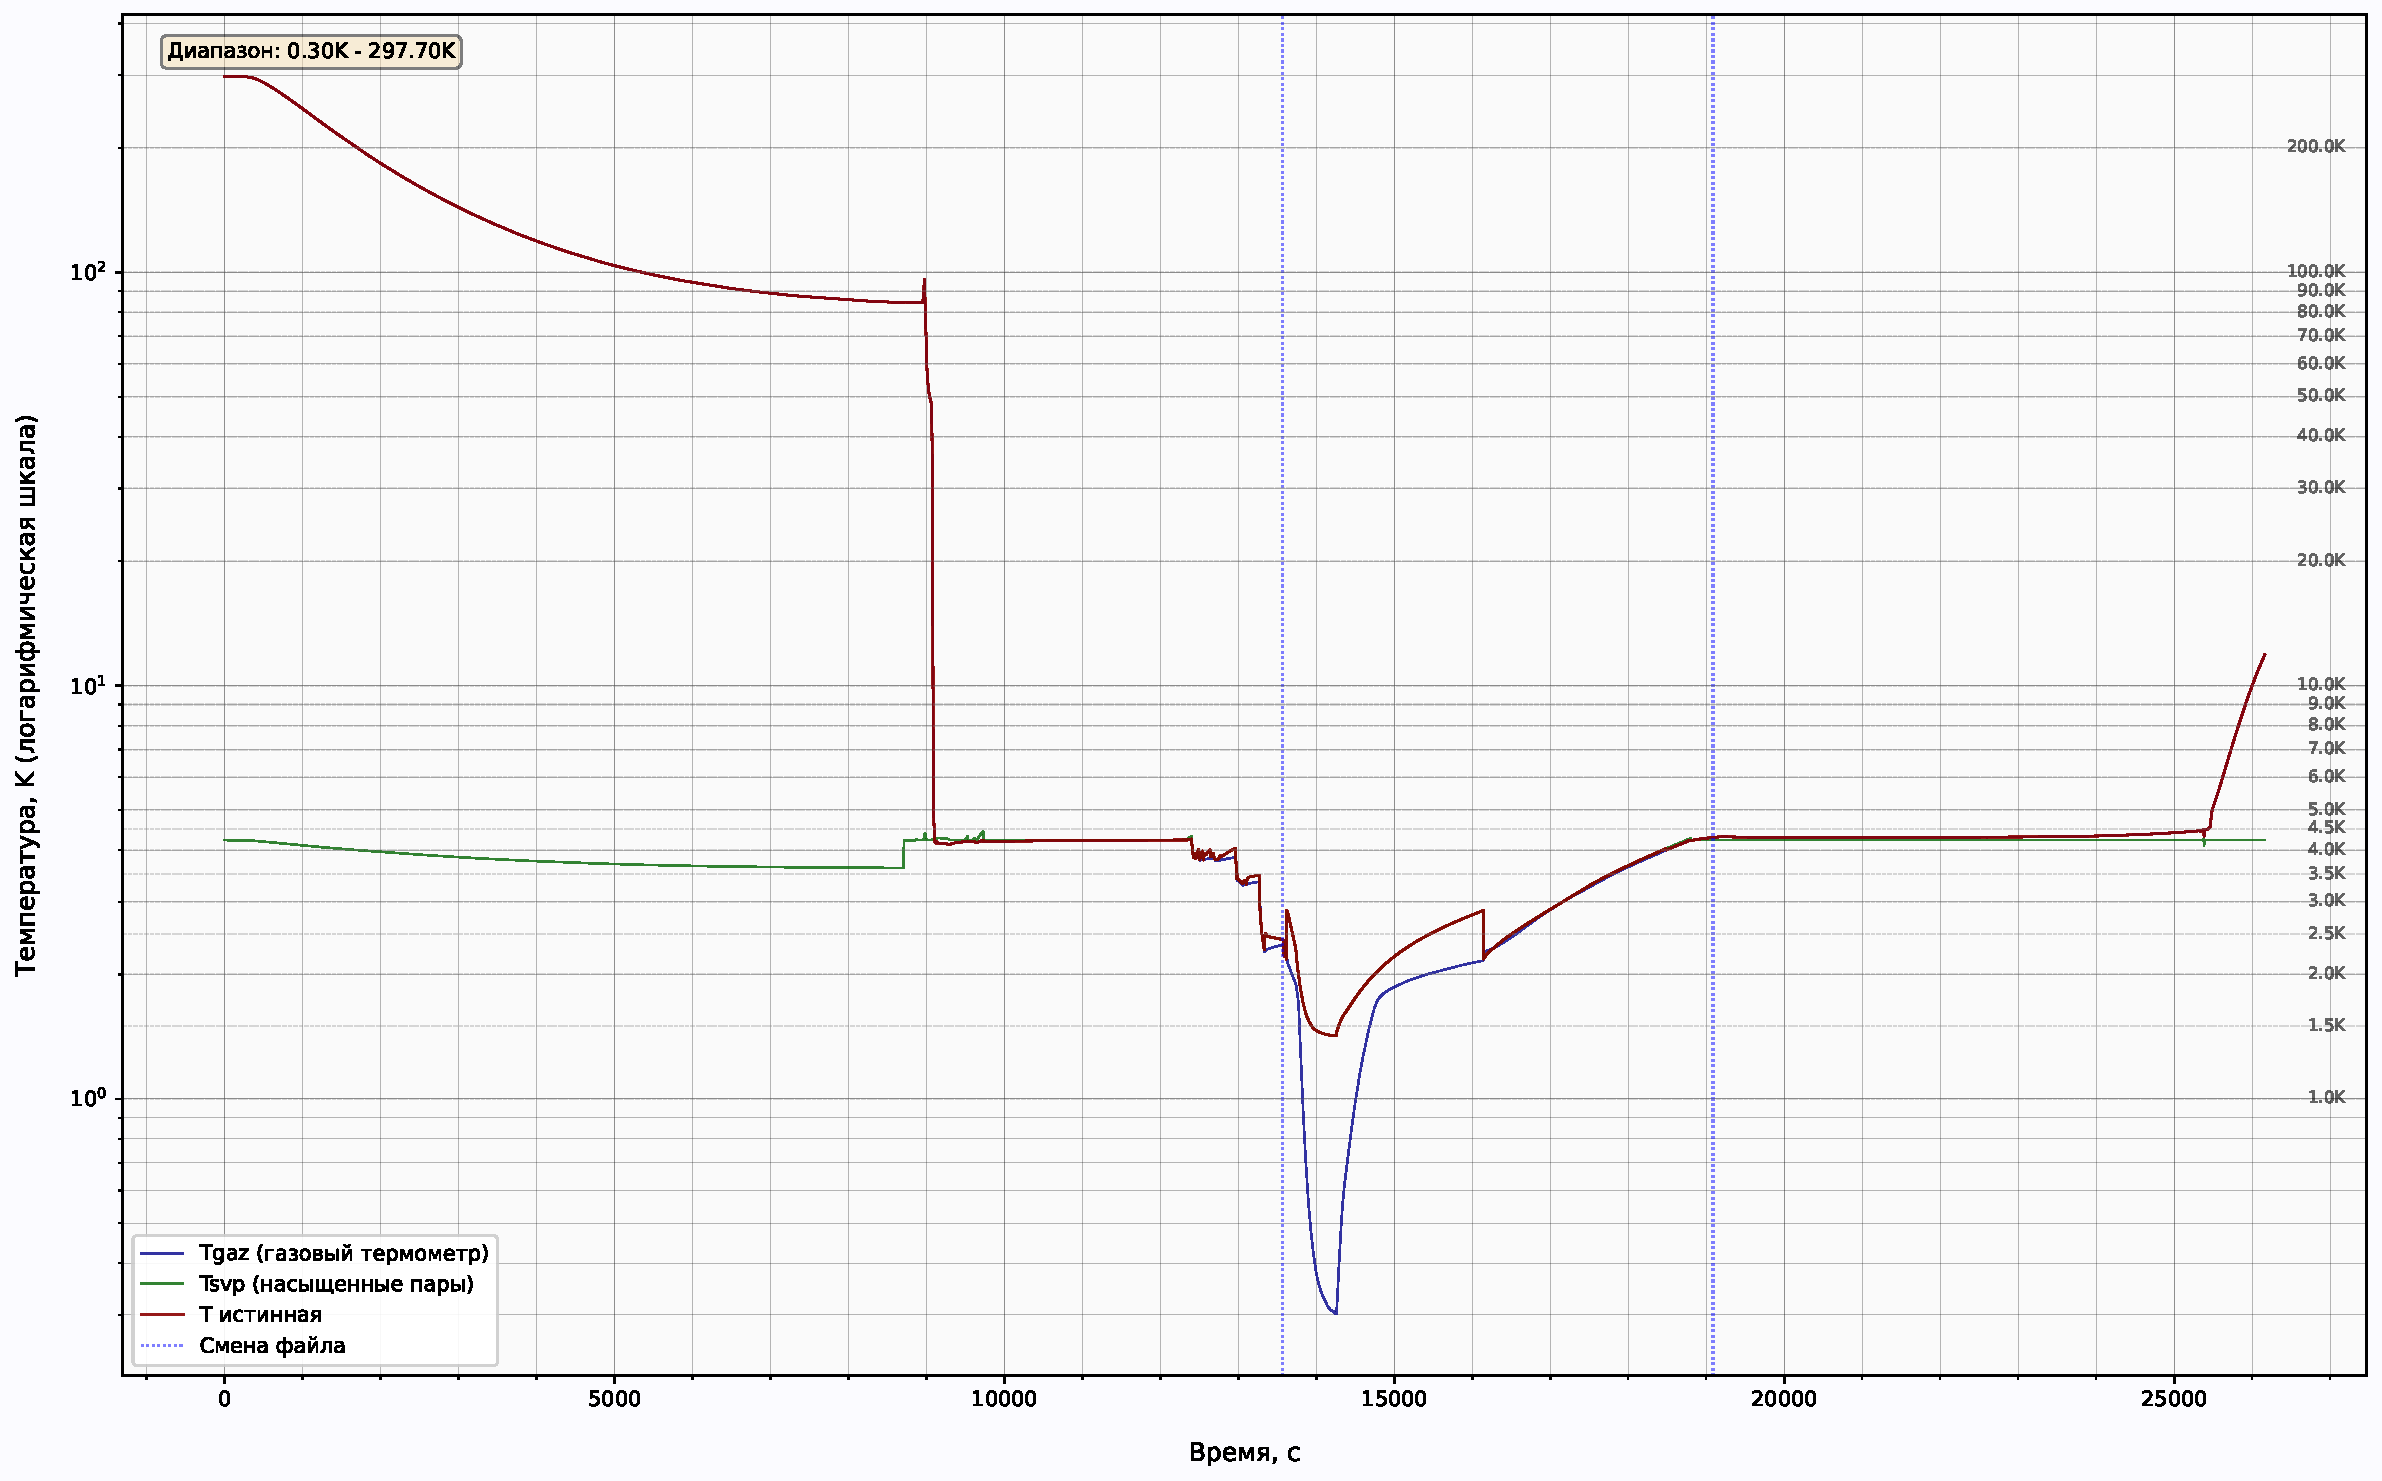
\includegraphics[width=\linewidth]{temperatures.pdf}
    \caption{Зависимость давлений в криостате и газовом термометре от времени на протяжении эксперимента}
\end{figure}

\begin{enumerate}
    \item Криостат остался заполнен газообразным гелием из дьюара после заполнения газового термометра. Залили жидкий азот во внешний дьюар.
    \item Криостат охладился до \(T < 90\,\text{К}\). Открыли гелиевую сеть.
    \item Начало заливки жидкого \(^4\text{He}\), большое количество неравновесных процессов, которые и вызывают скачки давления в криостате.
    \item Криостат залит, \(T = 4.2\,\text{К}\).
    \item Начало откачки \(^4\text{He}\). Во время откачки она два раза прекращается на небольшое время. Возможно это было связано с воздействием на систему из соседней установки или некорректной работой пневматики насоса.
    \item Точка сверхтекучего перехода (для \(^4\text{He}\) это \(2.16\,\text{К}\)).
    \item Точка конденсации гелия в газовом термометре, (\(P_{\text{Газ.терм.}} = P_{\text{SVP}}\))).
    \item Начало изохорного отогрева.
    \item Точка кипения гелия в газовом термометре (\(P_{\text{Газ.терм.}} = P_{\text{SVP}}\))).
    \item Отогрев до \(T = 4.2\,\text{К}\). Переключение криостата на гелиевую систему. Азотный дьюар вмерз, поэтому был убран позже.
\end{enumerate}
\subsection*{Газовый термометр}

\begin{figure}[h]
    \centering
    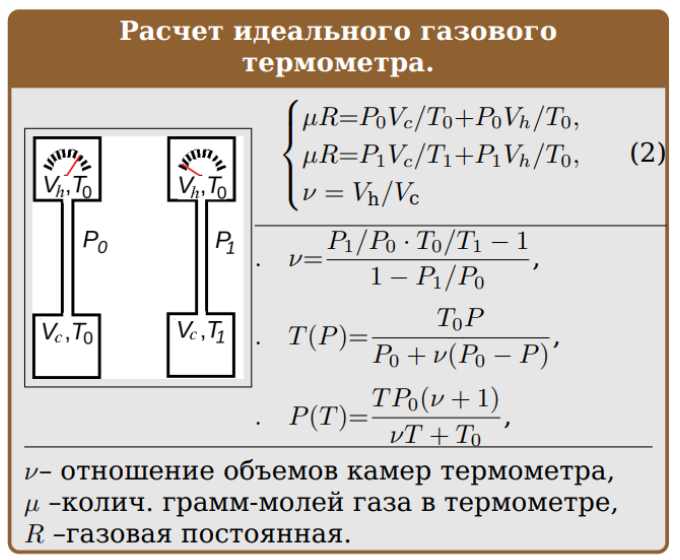
\includegraphics[width=0.6\linewidth]{gasterm.png}
    \caption{Калибровка газового термометра: Газовый термометр представляет собой два слабо сообщающихся объёма, в которых давление одинаково, а температуры разные: в верхнем — комнатная, а в нижнем — температура внутри криостата. Отсюда, считая гелий при соответствующих температурах идеальным газом, по калибровочным точкам получаем зависимость \(T(p)\).}
\end{figure}
При установившейся температуре жидкого гелия давление в газовом термометре составляло \(P_1 = 31.3\,\text{Торр}\). Зная, что при комнатной \(T_0 = 298\,\text{К}\) давление составляло \(P_0 = 771\,\text{Торр}\), можно произвести калибровку газового термометра. До достижения температуры гелия во время эксперимента использовалась точка кипения азота.

Стоит отметить, что данный термометр перестает работать при конденсации гелия, так как начинает меняться количество газообразного гелия (это произойдет примерно при 4.2 К). Этим мотивировано использование и другого типа термометра.

\subsection*{Термометр по давлению насыщеных паров}
Измерение температуры поверхности жидкого гелия по давлению его насыщенных паров относится к абсолютным методам и определяется международной шкалой температуры ITS-90 в диапазоне \(1.2\)–\(5\,\text{K}\) формулой с табулированными коэффициентами:

\[
T[\text{К}] = A_0 + \sum_{n=1}^{9} A_n \left[ \ln\left( \frac{P}{P_\text{Па}} \right) - B \right]^n,
\]


\section{Результаты}

Сразу стоит рассказать о фильтрации измеренных данных. Были отфильтрованы выходы измерительных приборов за пределы, строки с пустыми значениями. Были отфильтрованы точки с нулевым напряжением на генераторе, точки, в которых измерялся ВАХ, не использовались для зависимости $R(t)$, на зависимости $R(T)$ изображены серым цветом.
 
Измерения проводились при выставленном напряжении на источнике в 0.1 В, но из-за смещенного нуля оно оказалось меньше - около 0.04 В, что давало токи около 0.2 мкА, что все равно оказалось большим значением, что будет видно позже.
\begin{figure}[H]
    \centering
    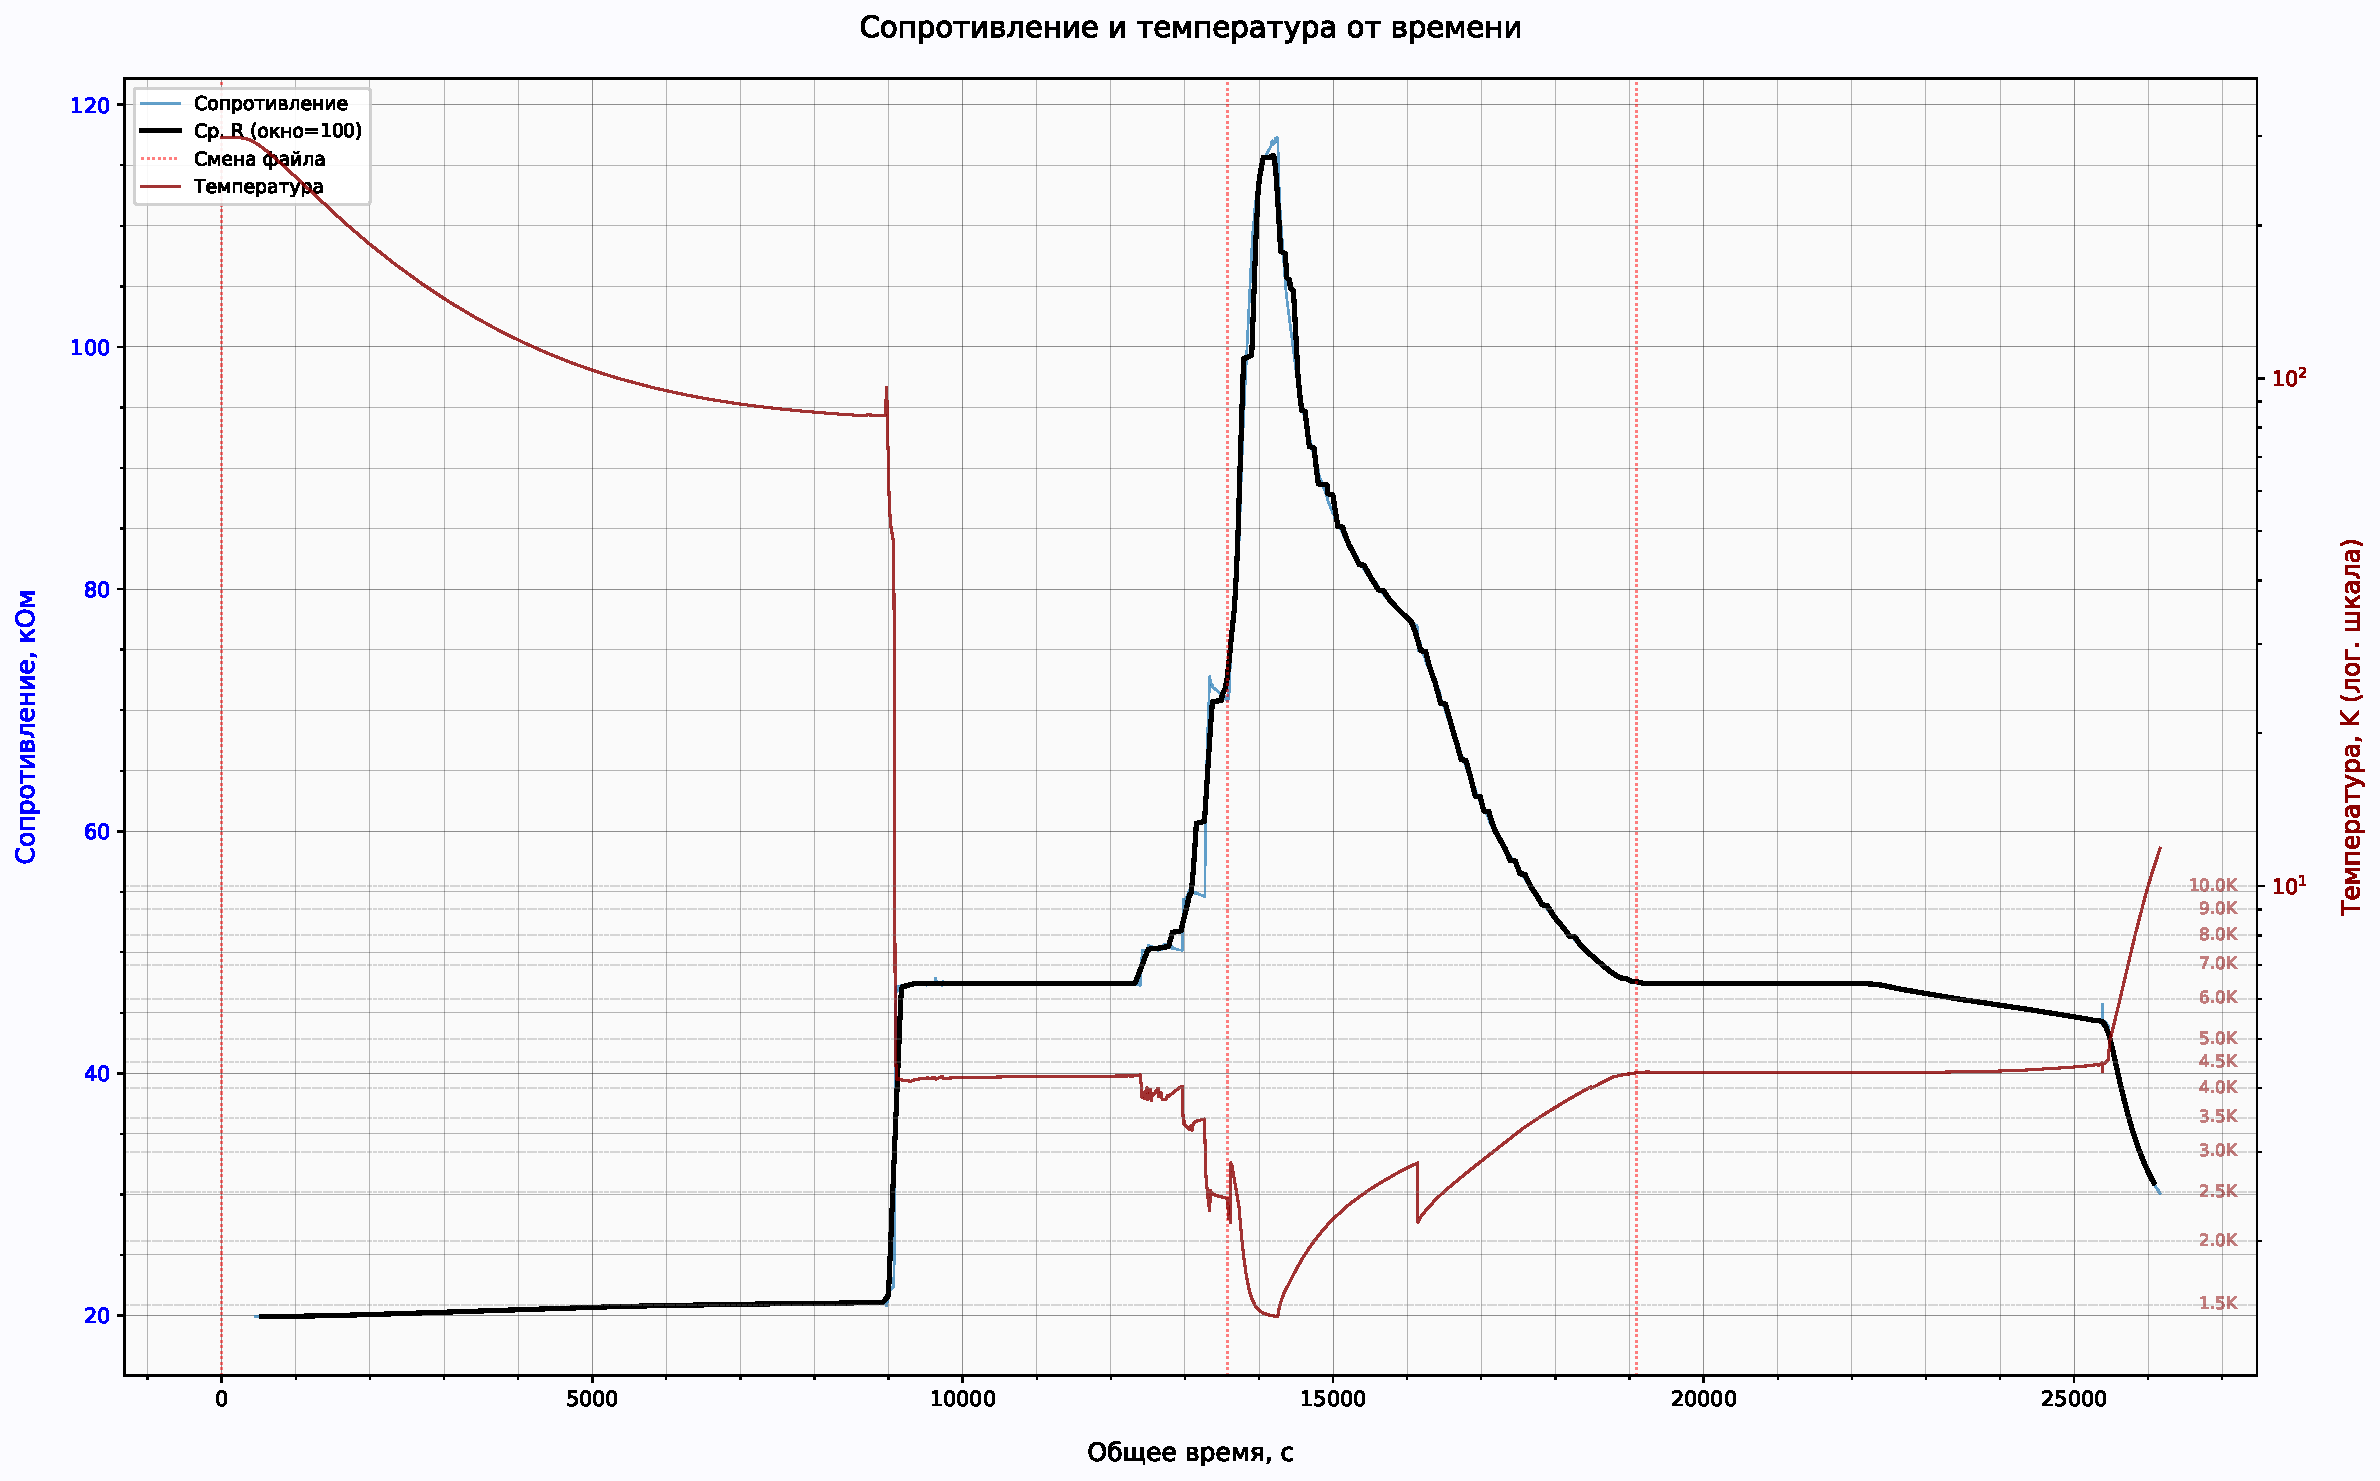
\includegraphics[width=\linewidth]{R_and_T.pdf}
    \caption{Зависимость напряжения и температуры на образце от времени}
\end{figure}

Ниже приведены ВАХ образца при гелиевых температурах, снятые на отогреве (там меньше сдвиг от нагрева образца и меньше изменение температуры во время измерения)

\begin{figure}[H]
    \centering
    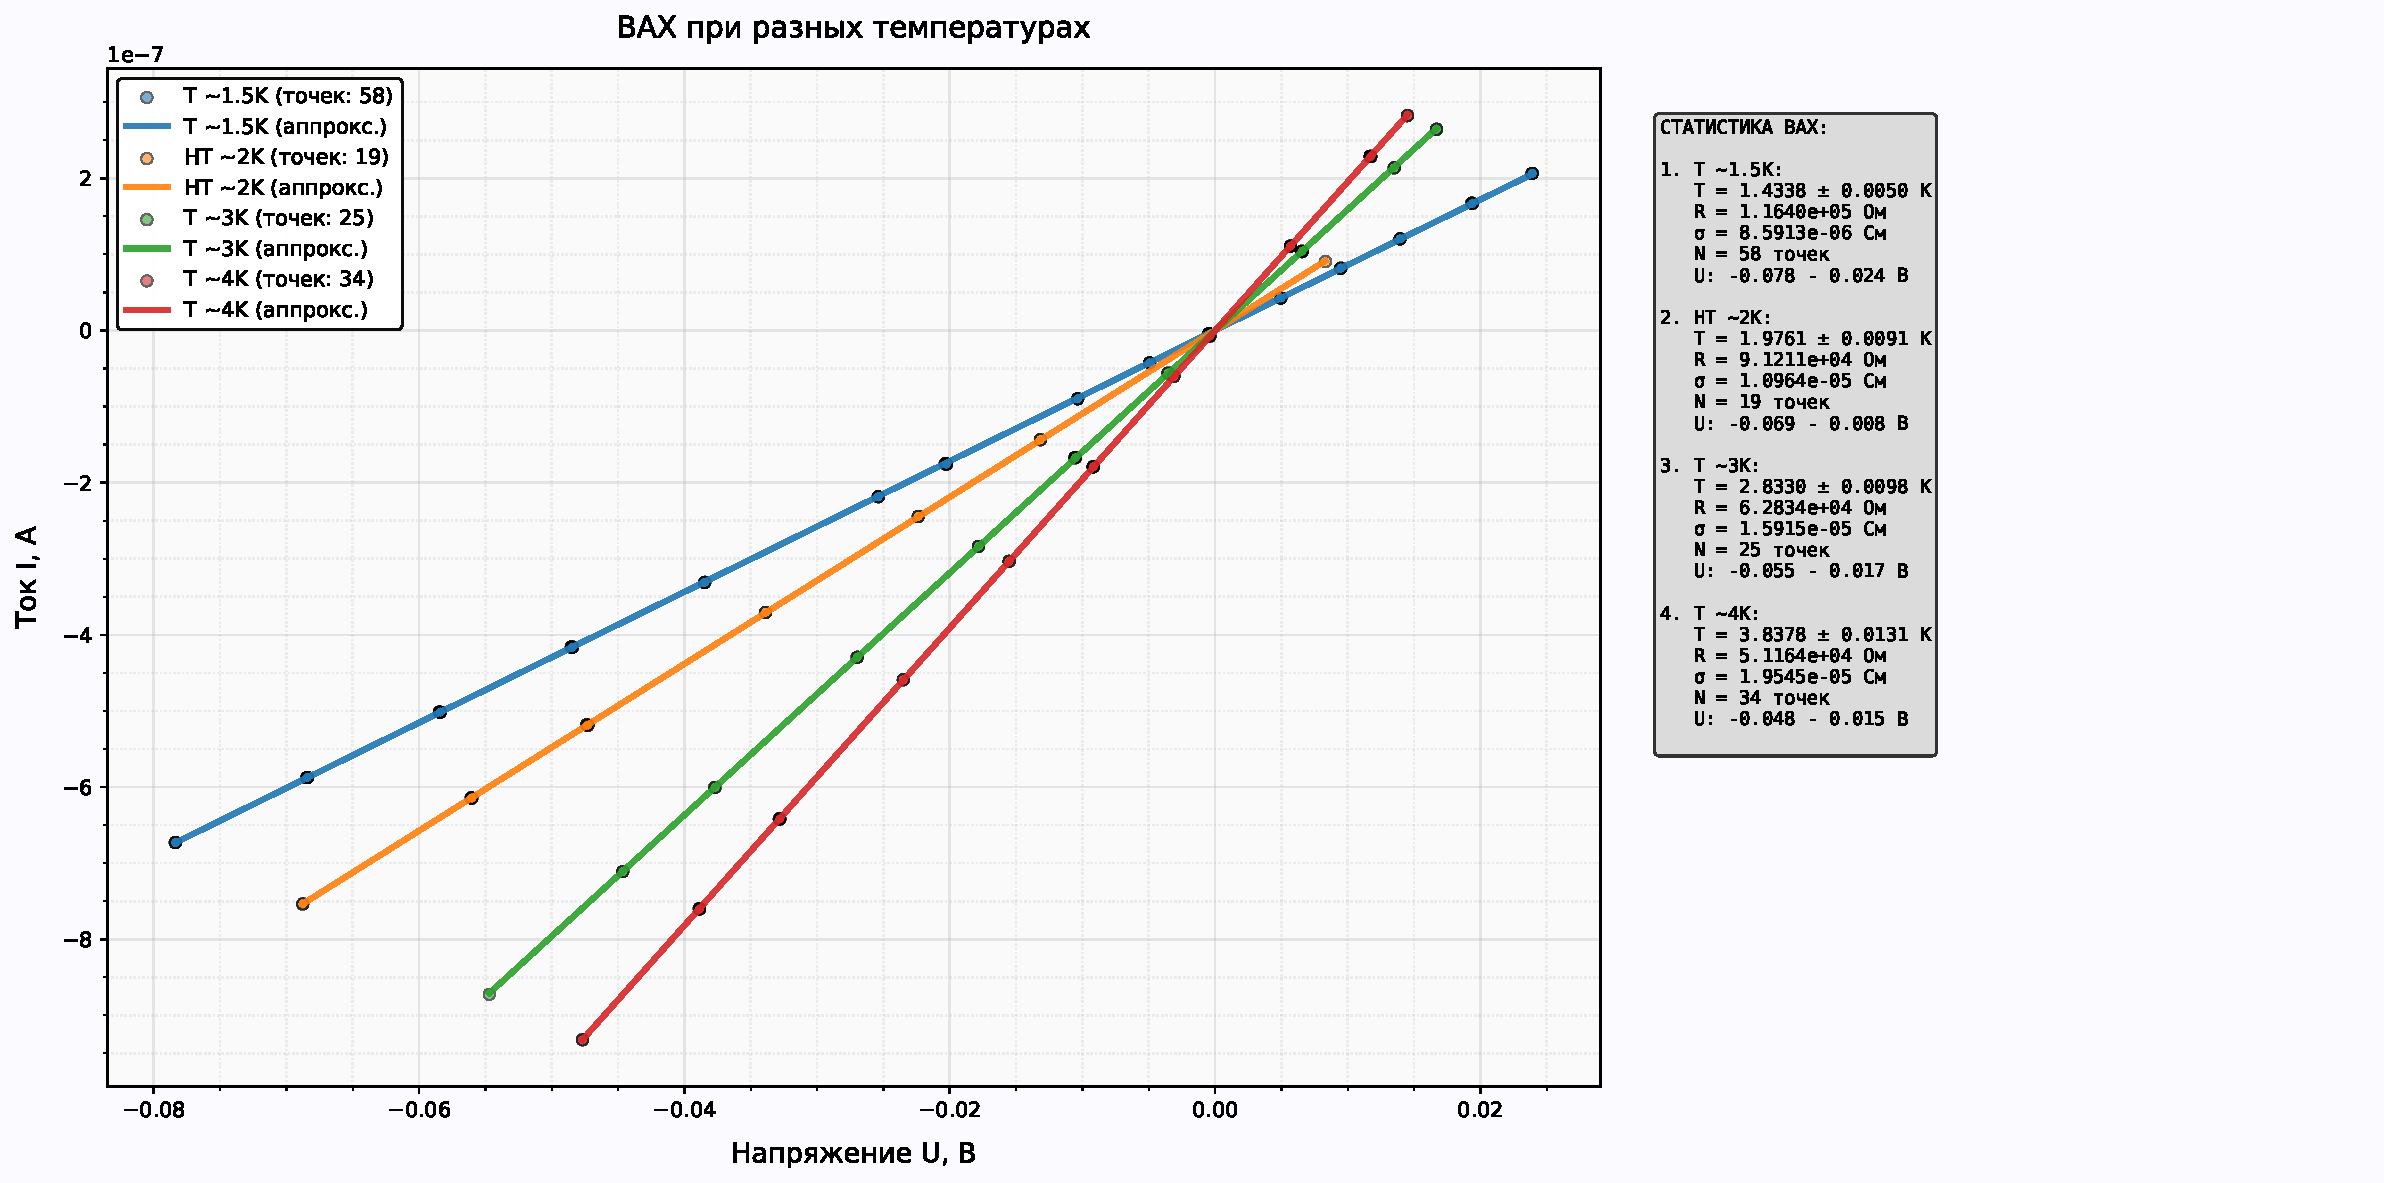
\includegraphics[width=\linewidth]{iv.pdf}
    \caption{ВАХ образца}
\end{figure}
ВАХ оказались линейными, как и ожидалось.

По результатам измерений были также получена зависимость сопротивления рутениевого образца от температуры:

\begin{figure}[H]
    \centering
    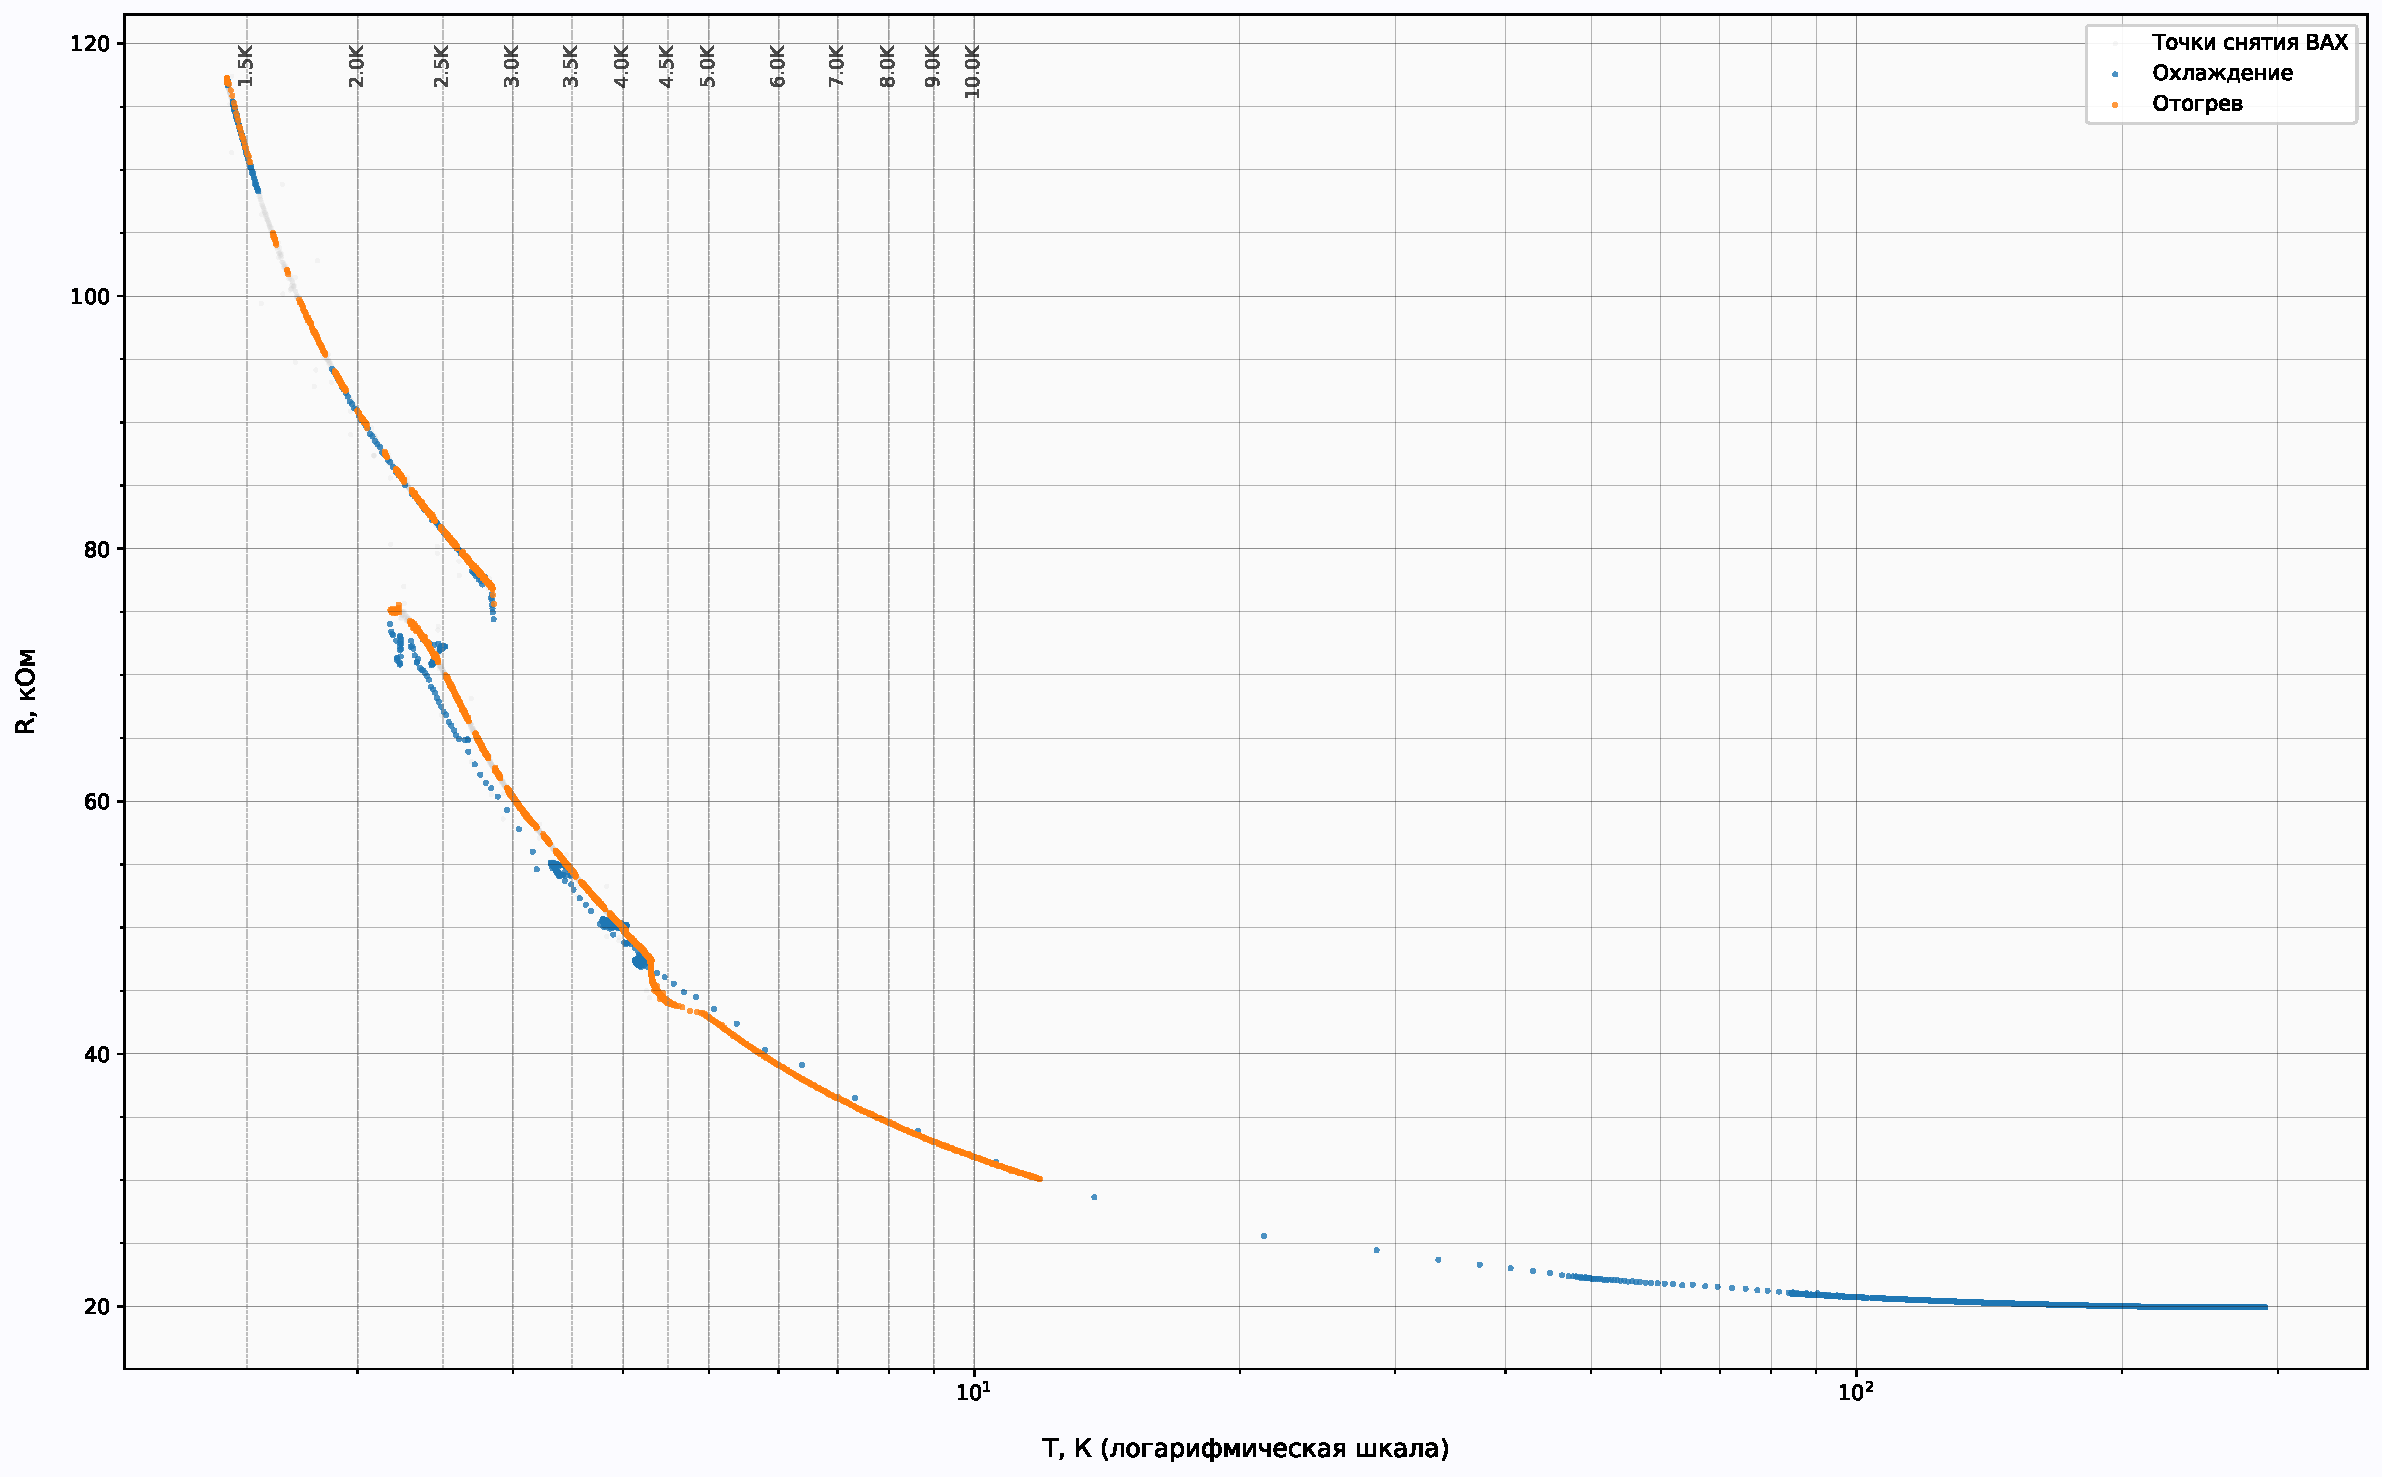
\includegraphics[width=\linewidth]{RvsT.pdf}
    \caption{Зависимость сопротивления образца от температуры}
\end{figure}

Как можно увидеть, помимо ожидаемого увеличения температуры при охлаждении образца, график содержит некоторое количество аномалий. Их причина - нагрев образца, из-за которого его температура отличается от температуры термометров. По этой причине сверхтекучая часть графика (>75 кОм) оторвана от обычной фазы, так как там за счет сверхтекучести происходило идеальный теплоотвод. Это подкрепляется тем, что результаты полученные при нагревании и охлаждении в сверхтекучей фазе совпадают. В обычном состоянии же нагрев образца приводил к смещению графиков влево (то есть действительная температура на образце серьезно (~0.5К) привышает температуру на термометре. Так же, вероятно, и скорость установления теплового равновесия является недостаточной, тк кривая отогрева смещена вверх относительно кривой охлаждения.
Все это говорит о том, что для корректного использования такого образца в качестве термометра нужно уменьшить измерительные токи, улучшить теплоотвод или лучше термоизолировать образец от вставки.


\section{Итоги}

В работе была выполнена калибровка рутенневого образца, получен график \(R(T)\), совпадающий с ожиданиями. Показана способность использования такого вида термометра и продемонстрированы его слабые места в виде влияния перегрева. Сняты ВАХ, которые, как и ожидалось, линейны.


\end{document}